% ============================================================
%  CHAPITRE 4 — Section 3 : Augmentation par l'état de santé
%  (RB2(SoH_H2), RB2(SoH_bat), RB2(SoH_all))
% ============================================================

\section{Augmentation par l'état de santé}
\label{sec:soh_aware}

L'augmentation par l'état de santé se décline en deux leviers indépendants, selon le composant dont la connaissance est exploitée. Le premier module les offsets confiés aux composants hydrogène en fonction de leur propre SoH (stratégie \RBsohH)~; le second module la fenêtre d'usage de la batterie en fonction du SoH de celle-ci (stratégie \RBsohB). Cette section les développe successivement — en montrant au passage qu'une voie intermédiaire séduisante, le report de flux vers l'hydrogène piloté par le SoH de la batterie, constitue une impasse instructive — puis les cumule dans la stratégie \RBsohA.

% ------------------------------------------------------------
\subsection{Modulation des offsets hydrogène~: \RBsohH}
\label{subsec:rb2sohh2}
% ------------------------------------------------------------

\subsubsection{Principe}

La stratégie RB2 répartit la puissance selon une logique d'offset constant. Lorsque la demande nette est positive, une puissance d'offset $P_{\text{FC-offset}}$ est confiée à la pile à combustible et la batterie fournit le complément. En cas d'excès de production, l'électrolyseur absorbe un offset $P_{\text{ELY-offset}}$ et la batterie assure le reste. Cet offset constant limite les transitoires et les cycles de démarrage-arrêt, mais il reste calibré sur l'état neuf et sollicite les composants hydrogène de la même manière tout au long de leur vie.

Le chapitre précédent a établi que ce sont les composants hydrogène dont l'usure répond le plus directement à la règle de répartition. Pour la pile à combustible, les cycles de démarrage-arrêt dominent la dégradation. Pour l'électrolyseur, c'est le fonctionnement soutenu à forte puissance. La stratégie \RBsohH{} exploite cette observation en autorisant l'offset confié à chaque composant hydrogène à suivre son état de santé courant~: un composant proche du neuf assure son offset nominal, un composant usé voit son offset réduit, son effort étant reporté sur la batterie. L'intensité de cette modulation est propre à chaque composant et réglée selon son mécanisme de dégradation dominant, comme le précisera la formalisation.

Cet usage du SoH se distingue de l'usage réactif du chapitre précédent. L'approche réactive n'employait le SoH que pour actualiser les bornes physiques des composants, sans modifier la logique de répartition. \RBsohH{} injecte le SoH dans la répartition elle-même.

\subsubsection{Formalisation}

Le SoH de chaque composant est fourni par les outils de diagnostic du chapitre dédié, à une cadence au moins hebdomadaire, suffisante au regard des constantes de temps du vieillissement. L'offset confié à chaque composant hydrogène est rendu fonction de son état de santé estimé au travers d'un exposant de modulation~:
\begin{equation}
\label{eq:rb2soh_offset}
P_{\text{FC-offset}}(t) = \mathrm{SoH}_{\text{FC}}(t)^{\,\gamma_{\text{FC}}}\,P_{\text{FC-offset}}^{0},
\qquad
P_{\text{ELY-offset}}(t) = \mathrm{SoH}_{\text{ELY}}(t)^{\,\gamma_{\text{ELY}}}\,P_{\text{ELY-offset}}^{0},
\end{equation}
où $P_{\text{FC-offset}}^{0}$ et $P_{\text{ELY-offset}}^{0}$ sont les offsets nominaux à l'état neuf, $\mathrm{SoH}_{\text{FC}}, \mathrm{SoH}_{\text{ELY}} \in [\,\mathrm{SoH}_{\text{EoL}}, 1\,]$ les états de santé estimés, et $\gamma_{\text{FC}}, \gamma_{\text{ELY}} \geq 0$ deux exposants réglant l'intensité avec laquelle chaque offset suit le SoH. Cette mise à l'échelle est cohérente avec la définition même du SoH des composants hydrogène, qui est lui-même un rapport de puissances délivrables (chapitre dédié)~: un offset exprimé comme une fraction de la puissance nominale décroît alors naturellement avec le SoH. La logique de répartition de RB2 est inchangée par ailleurs~; seule l'amplitude des offsets évolue dans le temps.

L'exposant $\gamma$ généralise la stratégie de référence. Pour $\gamma_{\text{FC}} = \gamma_{\text{ELY}} = 0$, les facteurs valent $1$, les offsets restent figés à leur valeur nominale et \RBsohH{} coïncide exactement avec RB2~: la stratégie statique est ainsi un cas particulier de \RBsohH, ce qui satisfait la propriété de test nul et garantit que tout écart de performance est imputable à la seule modulation par l'état de santé. À mesure qu'un exposant croît, l'offset correspondant suit plus fortement la dégradation du composant~: à $\mathrm{SoH} = 0{,}9$, un exposant $\gamma = 0{,}5$ abaisse l'offset de $5\,\%$, un exposant $\gamma = 1$ de $10\,\%$ et un exposant $\gamma = 2$ de $19\,\%$. Réduire ainsi l'offset d'un composant usé diminue sa sollicitation moyenne~: l'électrolyseur travaille à plus faible puissance, levier direct sur sa dégradation dominante, et son effort est reporté sur la batterie, dont le cyclage augmente mais dont le remplacement est moins coûteux que celui des composants hydrogène.

\subsubsection{Réglage des exposants}
\label{subsec:rb2soh_tuning}

Les deux exposants $\gamma_{\text{FC}}$ et $\gamma_{\text{ELY}}$ ont été réglés par balayage, en minimisant le coût total unifié sur l'horizon complet de vingt-cinq ans (VoLL~$=3$~€/kWh). Ce balayage est conduit à socle optimisé — les offsets nominaux $P_{\text{FC-offset}}^{0}$ et $P_{\text{ELY-offset}}^{0}$ sont eux-mêmes pris à leur meilleure valeur constante ($c_{\text{FC}} = 0{,}440$, $c_{\text{ELY}} = 0{,}310$) — de sorte que le cas $\gamma_{\text{FC}} = \gamma_{\text{ELY}} = 0$ coïncide exactement avec le meilleur RB2 statique~; l'écart de coût mesuré est ainsi \emph{purement attribuable} à la modulation par le SoH. Le Tableau~\ref{tab:rb2soh_gamma} en rapporte un extrait représentatif.

\begin{table}[h!]
\centering
\caption{Effet des exposants de modulation sur les indicateurs (balayage à socle optimal $c_{\text{FC}} = 0{,}440$, $c_{\text{ELY}} = 0{,}310$~; VoLL~$=3$~€/kWh). L'électrolyseur porte le gain de durabilité (dégradation)~; une modulation modérée de la pile à combustible parachève le compromis sur le coût total via la fiabilité. Le réglage retenu est en gras.}
\label{tab:rb2soh_gamma}
\begin{tabular}{ccccc}
\hline
$\gamma_{\text{FC}}$ & $\gamma_{\text{ELY}}$ & LPSP [\%] & Dégradation [k€] & Coût total [k€] \\
\hline
$0$ & $0$ & 2,59 & 58,85 & 80,11~(= RB2) \\
$0$ & $1$ & 2,81 & 57,37 & 80,44 \\
$0$ & $2$ & 3,08 & 54,46 & 79,76 \\
$\mathbf{1}$ & $\mathbf{2}$ & \textbf{2,91} & \textbf{54,91} & \textbf{78,77} \\
$2$ & $2$ & 2,99 & 55,36 & 79,90 \\
\hline
\end{tabular}
\end{table}

Deux enseignements se dégagent, qui tiennent directement à la nature des mécanismes de dégradation dominants identifiés au chapitre précédent. D'une part, moduler l'offset de l'électrolyseur ($\gamma_{\text{ELY}}$ croissant) abaisse nettement le coût de dégradation, de $58{,}85$ à $54{,}46$~k€ pour $\gamma_{\text{ELY}} = 2$~: l'usure de l'électrolyseur étant portée par le fonctionnement soutenu à forte puissance, réduire son offset agit directement sur sa cause dominante. C'est l'électrolyseur qui porte l'intégralité du gain de \emph{durabilité}. D'autre part, moduler l'offset de la pile à combustible ($\gamma_{\text{FC}}$ croissant) ne réduit pas le coût de dégradation — il le laisse quasiment inchangé, voire le relève légèrement — ce qui est cohérent avec une usure de la pile dominée par les cycles de démarrage-arrêt et non par le niveau de puissance. Sa modulation n'agit donc pas sur la durabilité, mais une valeur modérée $\gamma_{\text{FC}} = 1$ récupère en revanche une fraction de fiabilité (LPSP ramenée de $3{,}08$ à $2{,}91\,\%$), ce qui abaisse le coût total unifié.

Le réglage retenu combine ces deux effets~: $\gamma_{\text{ELY}} = 2$, une modulation marquée de l'électrolyseur qui porte le gain de durabilité, et $\gamma_{\text{FC}} = 1$, une modulation modérée de la pile à combustible qui optimise la composante fiabilité du coût total. Ce couple minimise le coût total unifié à $78{,}77$~k€, soit un gain \emph{pur} attribuable au SoH de $1{,}34$~k€ ($-1{,}67\,\%$) par rapport au meilleur RB2 statique ($80{,}11$~k€). Ce gain, plus modeste qu'il n'y paraîtrait face à un RB2 non optimisé, est la mesure honnête de l'apport propre du diagnostic une fois le socle lui-même réglé au mieux.

\subsubsection{Résultats}

La stratégie \RBsohH{} a été simulée dans le cadre du chapitre précédent et comparée à la référence RB2 dans le plan de Pareto. Les indicateurs agrégés sont reportés dans le Tableau~\ref{tab:rb2soh_results} et le positionnement dans le plan de Pareto à la Figure~\ref{fig:pareto_rb2soh}.

\begin{table}[h!]
\centering
\caption{Performances de \RBsohH{} comparées au meilleur RB2 statique (best-vs-best, VoLL~$=3$~€/kWh).}
\label{tab:rb2soh_results}
\begin{tabular}{lcccc}
\hline
Stratégie & LPSP [\%] & Coût de dégradation [k€] & Coût total [k€] & $\Delta$ total \\
\hline
RB2 (référence) & 2,59 & 58,85 & 80,11 & --- \\
\RBsohH{}       & 2,91 & 54,91 & 78,77 & $-1{,}67\,\%$ \\
\hline
\end{tabular}
\end{table}

La modulation par l'état de santé abaisse le coût de dégradation de $58{,}85$~k€ à $54{,}91$~k€, soit environ $-6{,}7\,\%$, en déchargeant l'électrolyseur vieillissant sur la batterie pour ralentir son usure et espacer les remplacements. Cet allègement se paie par une hausse de la LPSP, de $2{,}59\,\%$ à $2{,}91\,\%$~; nette, l'opération reste gagnante sur le coût total unifié, qui passe de $80{,}11$~k€ à $78{,}77$~k€ ($-1{,}67\,\%$). \RBsohH{} échange ainsi de la fiabilité contre de la durabilité de manière avantageuse~: son point de fonctionnement franchit, dans le plan de Pareto, une droite d'iso-coût unifié plus basse que le meilleur RB2 statique.

\begin{figure}[h!]
    \centering
    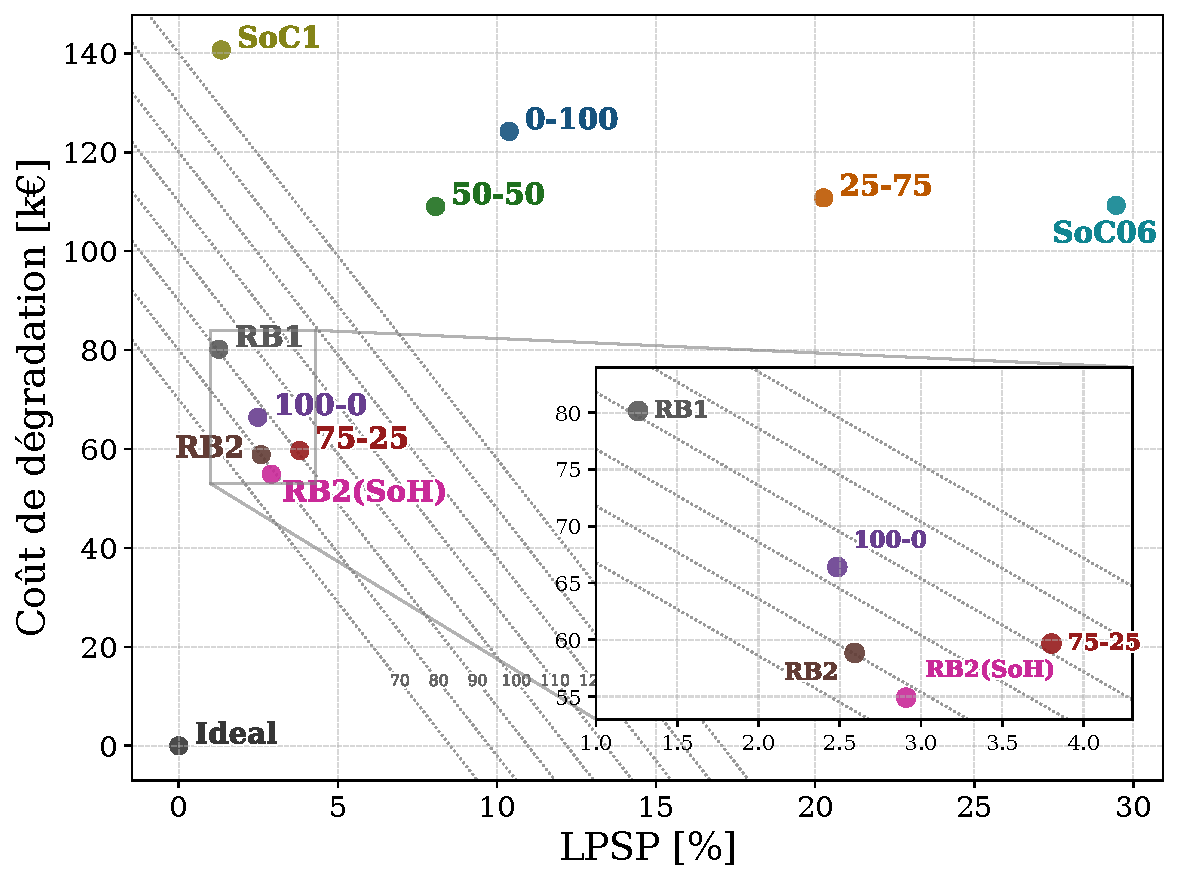
\includegraphics[width=\linewidth]{Chapitre 3/SoH/Figures/pareto_soh_isocost.pdf}
    \caption{Positionnement de \RBsohH{} dans le plan de Pareto LPSP--coût de dégradation, parmi le panel de stratégies du chapitre précédent, avec agrandissement sur l'amas RB2 (encart). Les droites pointillées grises sont les lignes d'\emph{iso-coût total unifié}~: coût de dégradation augmenté de la valorisation de la LPSP au \textit{Value of Lost Load} (VoLL~$=3$~€/kWh), soit une pente de $8{,}2$~k€ par point de LPSP~; leur étiquette indique le coût total en k€. Passer d'une stratégie à une droite d'iso-coût plus basse améliore le compromis fiabilité--durabilité.}
    \label{fig:pareto_rb2soh}
\end{figure}
\FloatBarrier

L'effet de la modulation est visible sur les profils de puissance de la Figure~\ref{fig:rb2soh_profiles}, qui présentent l'évolution des puissances sur quinze ans ainsi qu'un agrandissement sur une semaine. La puissance de l'électrolyseur décroît au fil du temps à mesure que son SoH se dégrade, conséquence directe de la modulation~\eqref{eq:rb2soh_offset}, là où elle restait stationnaire sous RB2. La batterie absorbe le report d'effort correspondant.

\begin{figure}[h!]
    \centering
    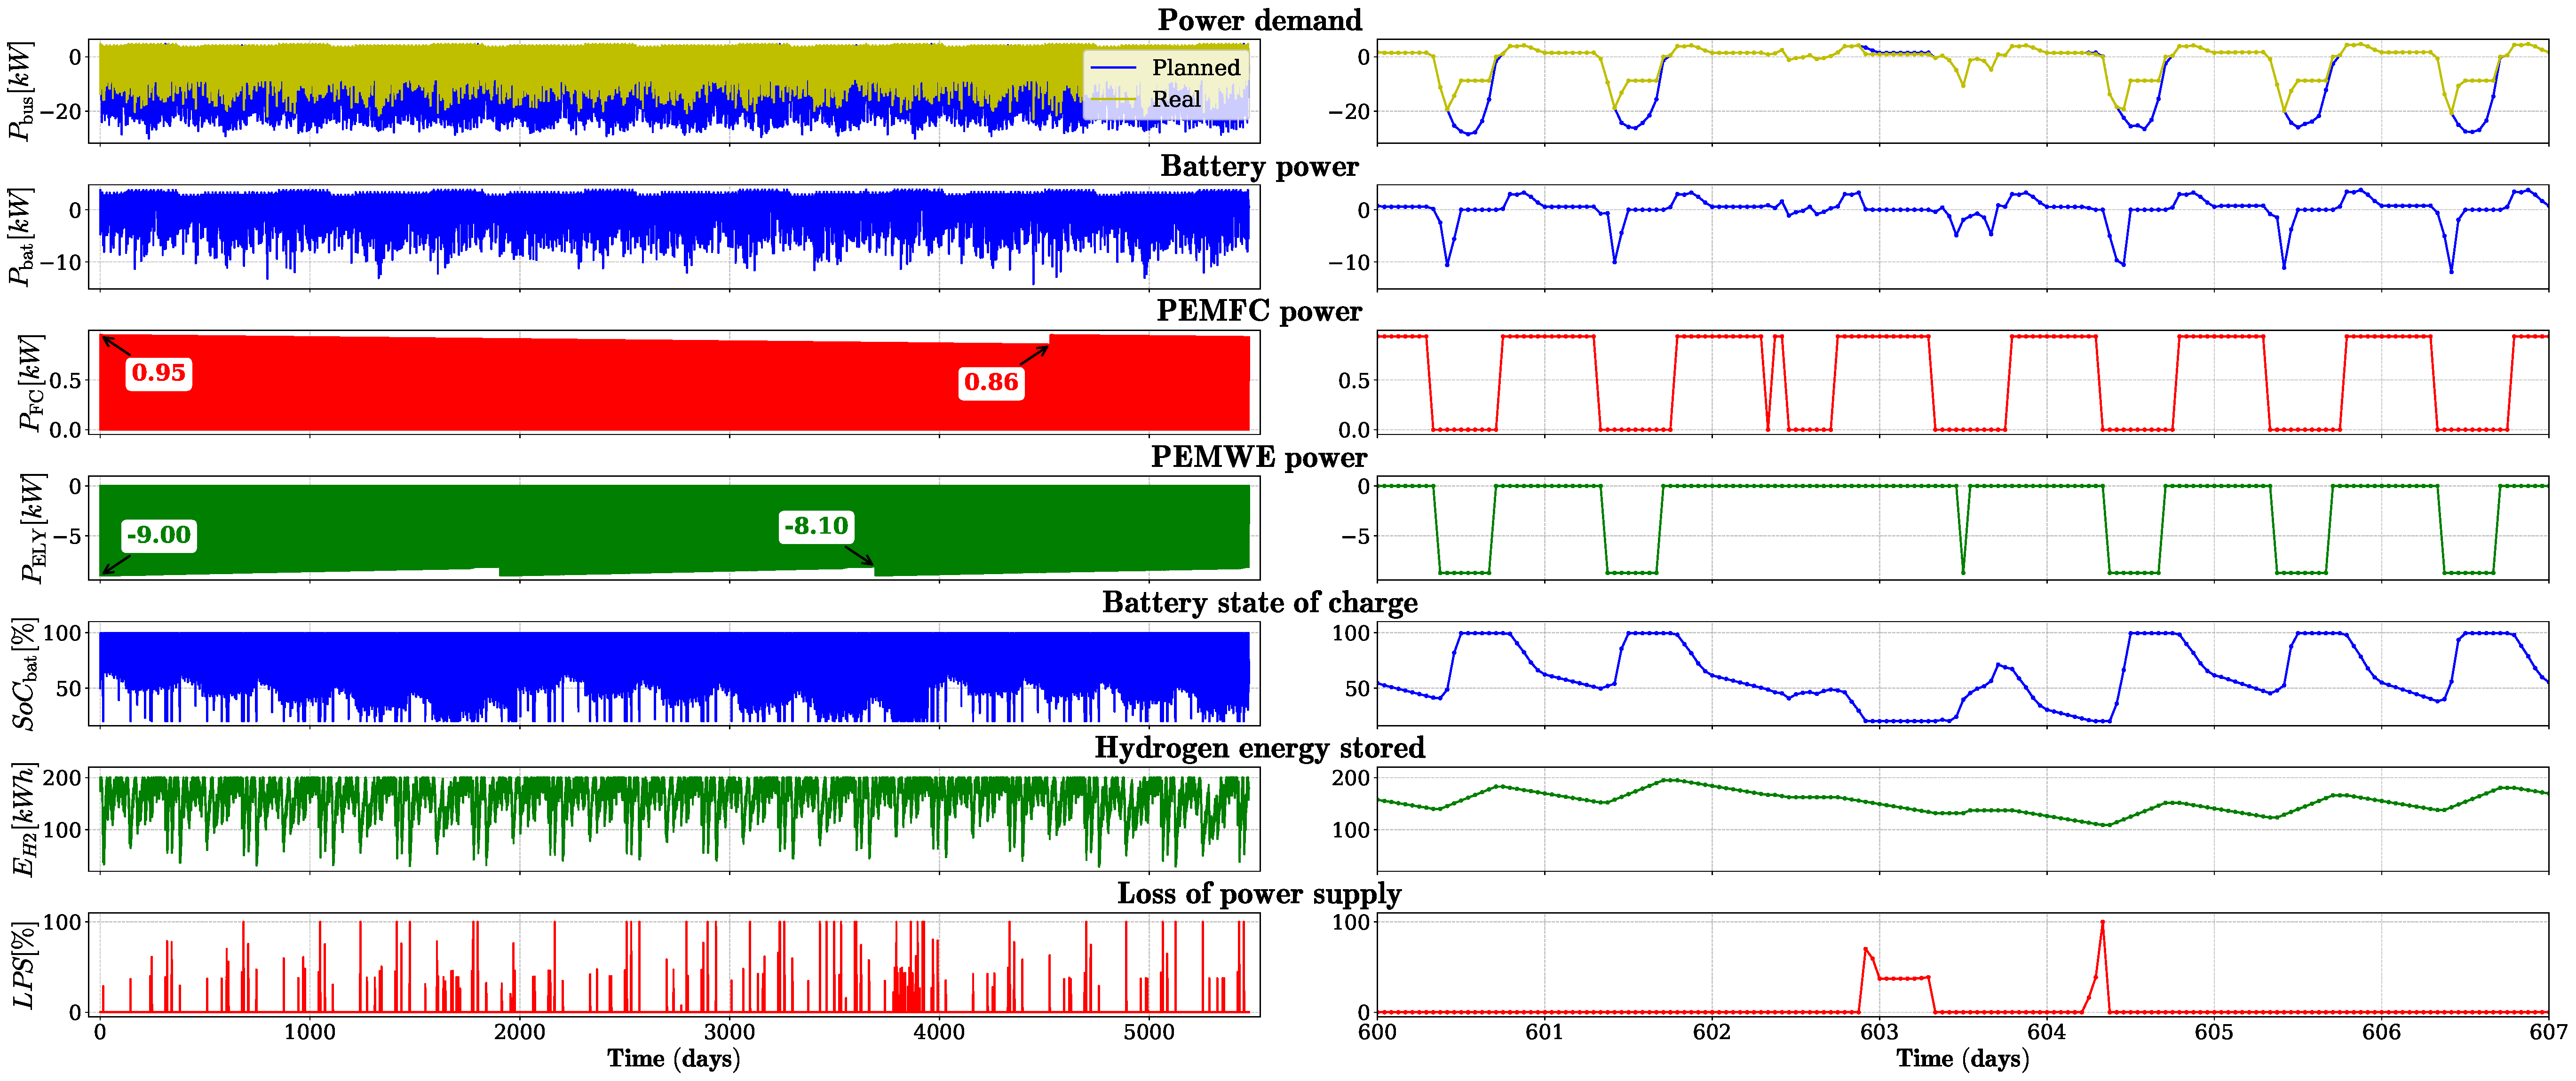
\includegraphics[width=\linewidth]{Chapitre 3/SoH/Figures/rb2soh_profiles.pdf}
    \caption{Profils de puissance sous \RBsohH{}~: simulation sur quinze ans (gauche) et agrandissement sur une semaine (droite).}
    \label{fig:rb2soh_profiles}
\end{figure}
\FloatBarrier

L'évolution du vieillissement et la décomposition des mécanismes de dégradation sont reportées à la Figure~\ref{fig:rb2soh_aging}. Les courbes de SoH font apparaître les remplacements périodiques des composants, et la répartition des mécanismes de dégradation des composants hydrogène y est détaillée. La réduction progressive de la sollicitation de l'électrolyseur se traduit sur sa durée de vie et sur le poids relatif de sa dégradation à forte puissance.

\begin{figure}[h!]
    \centering
    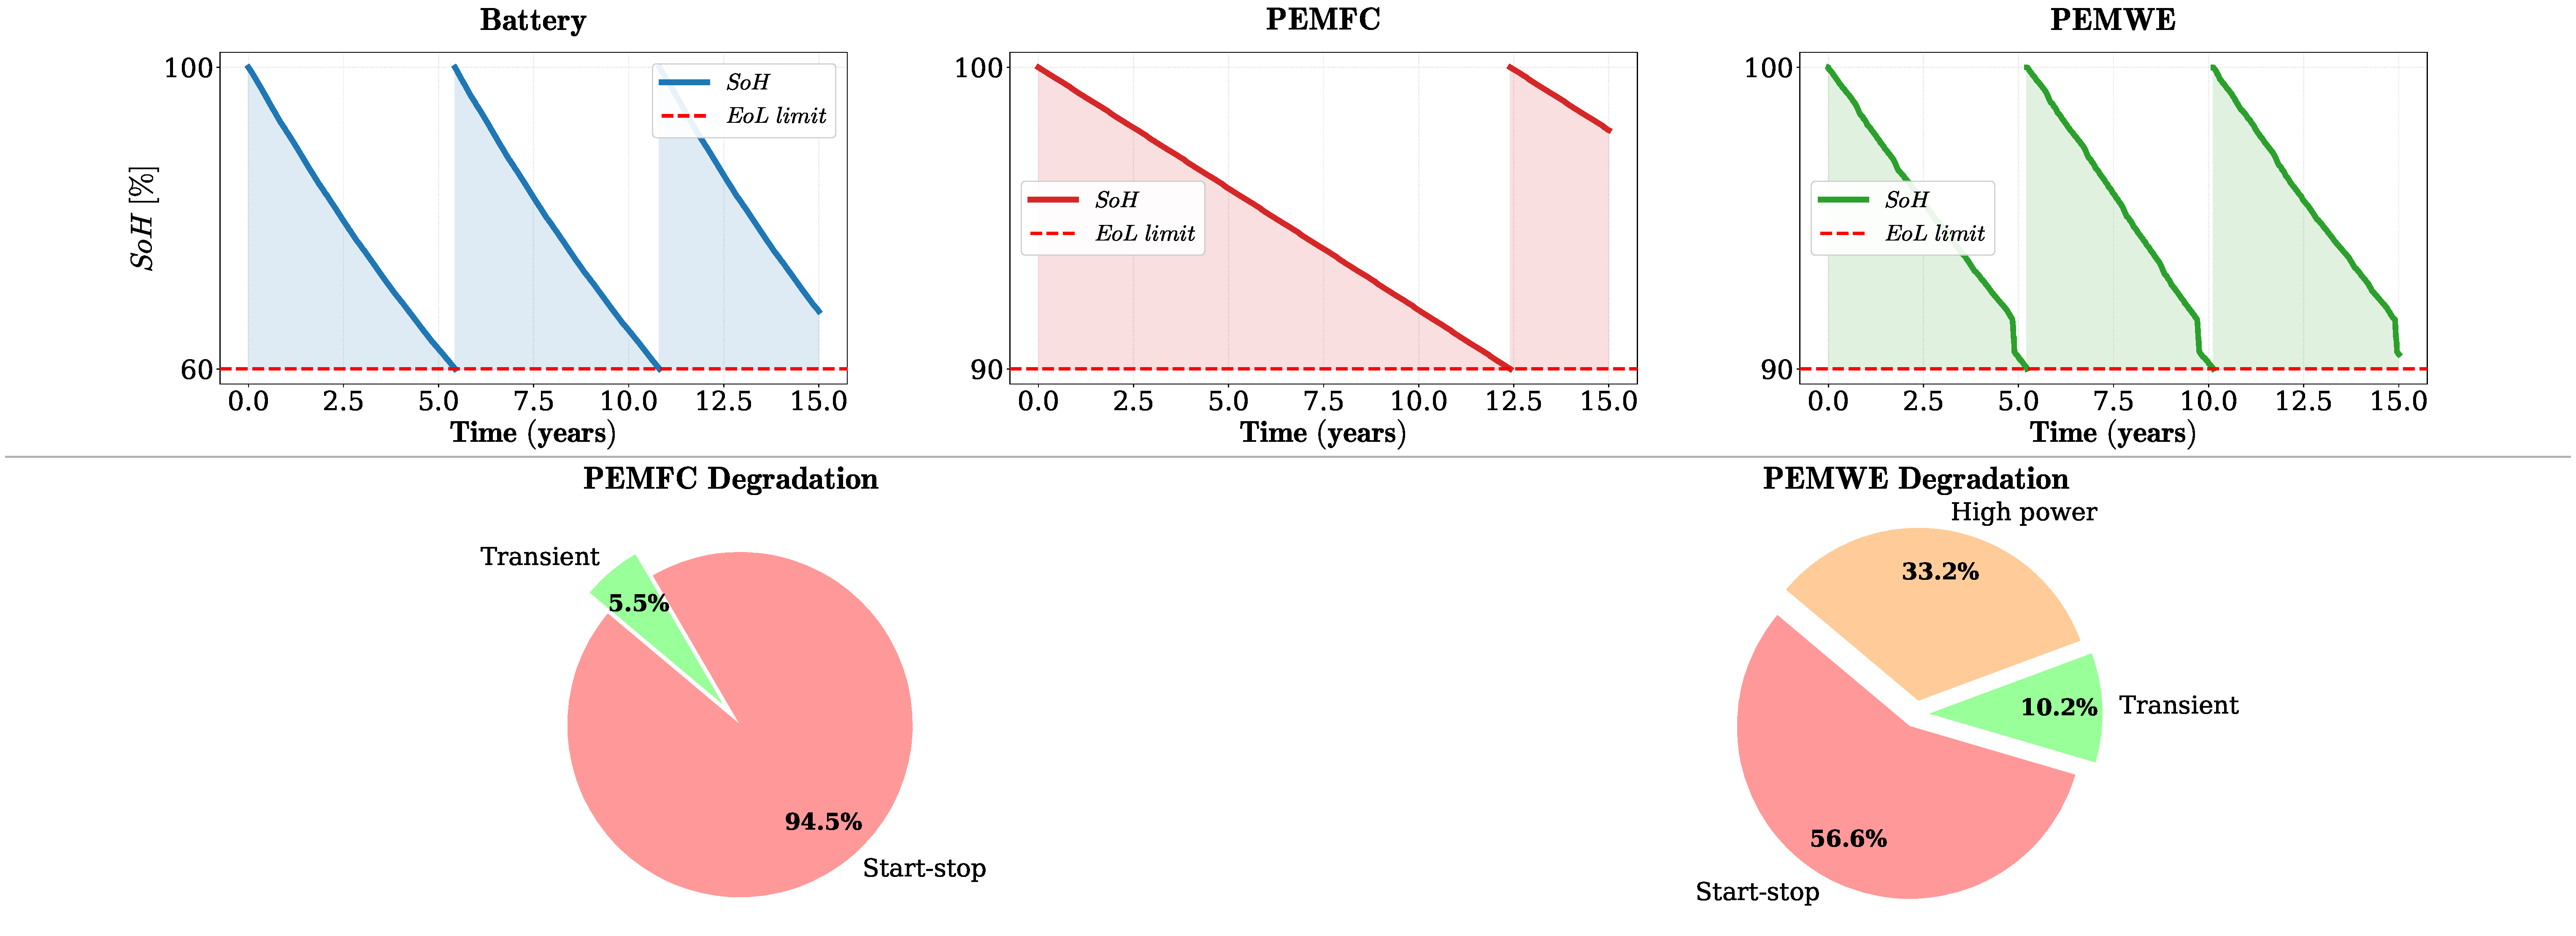
\includegraphics[width=\linewidth]{Chapitre 3/SoH/Figures/rb2soh_aging.pdf}
    \caption{Vieillissement sous \RBsohH{}~: évolution du SoH des composants (haut) et répartition des mécanismes de dégradation des composants hydrogène (bas).}
    \label{fig:rb2soh_aging}
\end{figure}
\FloatBarrier

% ------------------------------------------------------------
\subsection{Le gisement batterie}
\label{subsec:gisement_batterie}
% ------------------------------------------------------------

La stratégie \RBsohH{} n'exploite que le SoH des composants hydrogène~; celui de la batterie, pourtant également fourni par les outils de diagnostic, reste inutilisé dans la décision. Or, si les composants hydrogène sont ceux dont l'usure répond le plus directement à la règle de répartition, c'est la batterie qui pèse le plus lourd dans le coût de dégradation cumulé. Le Tableau~\ref{tab:decomposition_deg} en donne la décomposition sur l'horizon de vingt-cinq ans, obtenue en croisant les coûts de remplacement unitaires du cas d'étude et les durées de vie observées en simulation (environ cinq ans pour la batterie, douze pour la pile, treize pour l'électrolyseur sous RB2).

\begin{table}[h!]
\centering
\caption{Décomposition du coût de dégradation sur vingt-cinq ans (coûts de remplacement unitaires du cas d'étude, durées de vie observées sous RB2).}
\label{tab:decomposition_deg}
\begin{tabular}{lcccc}
\hline
Composant & Coût de remplacement [k€] & Vies sur 25 ans & Coût cumulé [k€] & Part \\
\hline
Batterie        & 7,0  & $\approx 5$   & $\approx 35$  & $\approx 63\,\%$ \\
Électrolyseur   & 9,3  & $\approx 1,9$ & $\approx 18$  & $\approx 32\,\%$ \\
Pile à combustible & 1,2 & $\approx 2,1$ & $\approx 2,5$ & $\approx 4\,\%$ \\
\hline
\end{tabular}
\end{table}

La batterie porte ainsi près des deux tiers du coût de dégradation~: elle constitue, mécaniquement, le premier gisement d'amélioration restant. Cette décomposition éclaire d'ailleurs rétrospectivement le faible enjeu de la modulation de la pile à combustible observé au balayage des exposants~: avec $4\,\%$ du coût, la pile n'offre structurellement presque rien à gagner en durabilité, quelle que soit la finesse de sa modulation.

Exploiter le SoH de la batterie se heurte cependant à une difficulté structurelle. Dans la logique de RB2, la batterie est la variable d'\emph{ajustement}~: elle absorbe le résidu de puissance que la chaîne hydrogène ne prend pas, et ne possède aucune consigne propre. La modulation d'offset de l'équation~\eqref{eq:rb2soh_offset} ne lui est donc pas transposable~: on ne peut pas « dérater » un composant qui n'a pas de consigne. Deux voies restent ouvertes~: déplacer du flux \emph{hors} de la batterie en remontant les offsets hydrogène quand elle vieillit, ou restreindre son \emph{domaine d'usage}. Les deux sont examinées ci-après~; seule la seconde s'avérera fructueuse, pour des raisons qui tiennent à la physique du modèle de dégradation de l'électrolyseur.

% ------------------------------------------------------------
\subsection{Une impasse instructive~: le report de flux vers l'hydrogène}
\label{subsec:cross_modulation}
% ------------------------------------------------------------

La première voie, dite de \emph{modulation croisée}, est le symétrique exact de \RBsohH{}~: lorsque la batterie vieillit, les offsets hydrogène sont \emph{remontés} pour que la chaîne hydrogène prenne une part croissante du transit d'énergie, la batterie cyclant d'autant moins~:
\begin{equation}
\label{eq:cross_modulation}
P_{\text{FC-offset}}(t) = \mathrm{SoH}_{\text{bat}}(t)^{-\beta_{\text{FC}}}\,P_{\text{FC-offset}}^{0},
\qquad
P_{\text{ELY-offset}}(t) = \mathrm{SoH}_{\text{bat}}(t)^{-\beta_{\text{ELY}}}\,P_{\text{ELY-offset}}^{0},
\end{equation}
avec $\beta_{\text{FC}}, \beta_{\text{ELY}} \geq 0$ (le cas $\beta = 0$ redonnant RB2, test nul préservé). L'arbitrage semble favorable sur le papier~: un kilowattheure cyclé par la batterie entame un réservoir de vie qui coûte $7$~k€ tous les cinq ans, quand l'électrolyseur du socle semble disposer de marge.

Le balayage de $(\beta_{\text{FC}}, \beta_{\text{ELY}})$ sur vingt-cinq ans dément sans appel cette intuition (Tableau~\ref{tab:cross_modulation})~: le coût total se dégrade de façon \emph{monotone} et massive dès la plus petite modulation, et l'optimum est $\beta = 0$, c'est-à-dire l'absence de levier.

\begin{table}[h!]
\centering
\caption{Balayage de la modulation croisée (report de flux vers l'hydrogène piloté par le SoH de la batterie, socle optimal, VoLL~$=3$~€/kWh)~: échec monotone, l'optimum est l'absence de modulation.}
\label{tab:cross_modulation}
\begin{tabular}{ccccc}
\hline
$\beta_{\text{FC}}$ & $\beta_{\text{ELY}}$ & LPSP [\%] & Dégradation [k€] & Coût total [k€] \\
\hline
$0$ & $0$      & 2,59 & 58,84 & 80,10~(= RB2) \\
$0$ & $0{,}25$ & 2,52 & 62,51 & 83,14 \\
$0$ & $0{,}5$  & 2,51 & 67,55 & 88,15 \\
$0$ & $1$      & 2,49 & 75,94 & 96,35 \\
$0{,}5$ & $0{,}5$ & 2,60 & 67,81 & 89,15 \\
$1$ & $1$      & 2,75 & 80,24 & 102,77 \\
\hline
\end{tabular}
\end{table}

L'explication tient à la forme à seuil du modèle de dégradation de l'électrolyseur PEM établi au chapitre précédent~: en dessous d'environ $30\,\%$ de la puissance maximale (soit \SI{1}{\ampere\per\centi\metre\squared}), les taux de génération de dégradation réversible et irréversible sont nuls~; ils croissent ensuite avec la charge. Or l'offset optimal du socle, $c_{\text{ELY}} = 0{,}310$, se situe précisément \emph{au genou de zéro-usure} de ce modèle~: l'électrolyseur du meilleur RB2 fonctionne quasi gratuitement en dégradation. Toute remontée de son offset — même de $9\,\%$, ce que produit $\beta_{\text{ELY}} = 0{,}25$ en fin de vie de batterie — le fait entrer dans la zone génératrice d'usure, dont le coût marginal écrase l'économie espérée sur la batterie ($+3{,}7$~k€ de dégradation dès $\beta_{\text{ELY}} = 0{,}25$, pour un gain de LPSP marginal). Côté pile, la remontée d'offset échoue par un autre canal~: elle draine le réservoir d'hydrogène plus vite, et la LPSP se dégrade.

Cette impasse a valeur d'enseignement, et éclaire rétrospectivement deux résultats. D'abord, l'optimum $c_{\text{ELY}} = 0{,}310$ du socle n'est pas un compromis numérique arbitraire~: c'est le plus grand offset — donc le plus d'hydrogène stocké et la meilleure fiabilité — qui maintient l'électrolyseur sous son genou de zéro-usure~; l'optimisation du chapitre précédent avait trouvé ce point physique sans le nommer. Ensuite, la modulation $\gamma_{\text{ELY}} > 0$ de \RBsohH{} s'interprète comme un \emph{asservissement implicite à ce genou}~: le seuil de $30\,\%$ étant défini par rapport à la puissance maximale \emph{vieillie}, qui décroît avec l'usure, un offset figé sur l'état neuf dériverait au-dessus du genou à mesure que l'électrolyseur vieillit~; la décroissance en $\mathrm{SoH}^{\gamma}$ l'y ramène. Plus généralement, dans un EMS dont le socle est déjà optimisé en coût, chaque organe opère près de son point d'usure minimale~: il n'existe pas de marge d'usure cachée à redéployer d'un composant vers un autre. Ce constat est conditionné par la forme à seuil du modèle de dégradation considéré~; pour une technologie d'électrolyseur s'usant dès les faibles charges, la modulation croisée pourrait conserver une marge.

% ------------------------------------------------------------
\subsection{La fenêtre de SoC vieillissante~: \RBsohB}
\label{subsec:rb2sohbat}
% ------------------------------------------------------------

La seconde voie ne déplace pas de flux~: elle restreint le domaine d'usage de la batterie là où celle-ci s'use le plus. Le modèle de dégradation de la batterie du chapitre précédent associe à chaque niveau de SoC une densité de dommage par unité de charge échangée, sensiblement plus élevée en zone haute de SoC. Le levier consiste alors à abaisser le plafond de SoC autorisé à mesure que la batterie vieillit~:
\begin{equation}
\label{eq:soc_ceiling}
\mathrm{SoC}_{\max}(t) = \mathrm{SoC}_{\max}^{0} - g\,\big(1 - \mathrm{SoH}_{\text{bat}}(t)\big),
\end{equation}
où $\mathrm{SoC}_{\max}^{0} = 0{,}995$ est le plafond nominal et $g \geq 0$ le gain de modulation~; le plancher de SoC est inchangé. Pour $g = 0$, la fenêtre reste figée et la stratégie coïncide avec RB2 (test nul)~; pour $g = 0{,}2$ et une batterie en fin de vie ($\mathrm{SoH}_{\text{bat}} = 0{,}7$), le plafond descend à $0{,}935$. Le cyclage est ainsi progressivement confiné hors de la zone de dommage haute, au prix d'une capacité utile réduite — donc d'un arbitrage durabilité--fiabilité, que le balayage du gain $g$ quantifie (Tableau~\ref{tab:socwin_sweep}).

\begin{table}[h!]
\centering
\caption{Balayage fin du gain $g$ de la fenêtre de SoC vieillissante (socle optimal, VoLL~$=3$~€/kWh). L'optimum $g^{*} = 0{,}2$ est en gras~; la cuvette est plate sur $[0{,}15\,; 0{,}30]$.}
\label{tab:socwin_sweep}
\begin{tabular}{ccccc}
\hline
$g$ & Plafond à l'EoL & LPSP [\%] & Dégradation [k€] & Coût total [k€] \\
\hline
$0$ (= RB2) & 0,995 & 2,59 & 58,84 & 80,10 \\
$0{,}05$    & 0,980 & 2,66 & 58,34 & 80,12 \\
$0{,}10$    & 0,965 & 2,70 & 57,82 & 79,99 \\
$0{,}15$    & 0,950 & 2,73 & 57,36 & 79,73 \\
$\mathbf{0{,}20}$ & \textbf{0,935} & \textbf{2,77} & \textbf{56,84} & \textbf{79,54} \\
$0{,}25$    & 0,920 & 2,84 & 56,27 & 79,59 \\
$0{,}30$    & 0,905 & 2,92 & 55,72 & 79,66 \\
$0{,}40$    & 0,875 & 3,03 & 54,87 & 79,72 \\
\hline
\end{tabular}
\end{table}

Trois lectures se dégagent. D'abord, le levier est \emph{gagnant}~: à l'optimum $g^{*} = 0{,}2$, le coût de dégradation baisse de $2{,}0$~k€ pour $0{,}18$ point de LPSP concédé, soit un gain net de $0{,}56$~k€ sur le coût total — davantage, on le verra, que l'apport du levier prévisionnel complet. C'est le premier gain de ce chapitre obtenu par la connaissance du SoH de la batterie. Ensuite, la dégradation décroît quasi linéairement avec $g$ tandis que la LPSP croît de façon convexe~: c'est la fiabilité qui fixe l'optimum, et au-delà de $g \approx 0{,}5$ la capacité retirée n'est plus compensable. Enfin, la cuvette est \emph{plate}~: tout $g$ dans $[0{,}15\,; 0{,}30]$ conserve l'essentiel du gain, si bien qu'une erreur de réglage de $\pm 50\,\%$ reste bénigne. Cette robustesse paramétrique, précieuse pour l'implémentation, contraste avec la sensibilité des seuils prévisionnels qui sera rencontrée à la section suivante.

% ------------------------------------------------------------
\subsection{Unification des leviers d'état de santé~: \RBsohA}
\label{subsec:rb2sohall}
% ------------------------------------------------------------

Les deux leviers validés agissent sur des ressources disjointes — les offsets de la chaîne hydrogène pour \RBsohH, la fenêtre d'usage de la batterie pour \RBsohB{} — et peuvent être cumulés. La stratégie unifiée \RBsohA{} applique simultanément la modulation~\eqref{eq:rb2soh_offset} avec $(\gamma_{\text{FC}}, \gamma_{\text{ELY}}) = (1, 2)$ et le plafond vieillissant~\eqref{eq:soc_ceiling} avec $g = 0{,}2$~: chaque composant y est piloté par son propre état de santé. Le Tableau~\ref{tab:rb2sohall} rapporte le balayage croisé.

\begin{table}[h!]
\centering
\caption{Cumul des deux leviers d'état de santé (socle optimal, VoLL~$=3$~€/kWh). Les gains s'additionnent à $93\,\%$ et les réglages optimaux de chaque levier sont inchangés en présence de l'autre.}
\label{tab:rb2sohall}
\begin{tabular}{lcccc}
\hline
Stratégie & $(\gamma_{\text{FC}}, \gamma_{\text{ELY}})\times g$ & LPSP [\%] & Dégradation [k€] & Coût total [k€] \\
\hline
RB2 (référence) & $(0,0)\times 0$      & 2,59 & 58,84 & 80,10 \\
\RBsohH{}       & $(1,2)\times 0$      & 2,91 & 54,91 & 78,76 \\
\RBsohB{}       & $(0,0)\times 0{,}2$  & 2,77 & 56,84 & 79,54 \\
\RBsohA{}       & $(1,2)\times 0{,}1$  & 3,04 & 53,89 & 78,83 \\
\RBsohA{}       & $\mathbf{(1,2)\times 0{,}2}$ & \textbf{3,11} & \textbf{52,87} & \textbf{78,34} \\
\RBsohA{}       & $(1,2)\times 0{,}3$  & 3,31 & 51,75 & 78,91 \\
\RBsohA{}       & $(1,2)\times 0{,}4$  & 3,45 & 50,91 & 79,23 \\
\hline
\end{tabular}
\end{table}

Deux propriétés de structure rendent ce cumul défendable au-delà de son chiffre. La première est l'\emph{additivité}~: les gains séparés valent $-1{,}34$~k€ (offsets hydrogène) et $-0{,}56$~k€ (fenêtre batterie), soit $-1{,}90$~k€ en cumul théorique~; le gain mesuré de la stratégie unifiée est de $-1{,}77$~k€, soit $93\,\%$ de la somme. Les deux leviers, agissant sur des ressources physiquement disjointes, ne se cannibalisent presque pas — la légère sous-additivité ($0{,}13$~k€) provenant du cumul de leurs coûts respectifs en LPSP dans les pires semaines. La seconde est la \emph{séparabilité des réglages}~: le couple $(\gamma_{\text{FC}}, \gamma_{\text{ELY}}) = (1,2)$ reste optimal en présence du plafond (les variantes $(0,2)$, $(2,2)$, $(1,3)$ et $(1,1)$ à $g = 0{,}2$ sont toutes dominées), et $g^{*} = 0{,}2$ reste optimal en présence des exposants, avec la même cuvette qu'en solo. Chaque levier se règle donc indépendamment sur sa propre grille, sans optimisation croisée — propriété précieuse pour transposer la démarche à un autre système.

\begin{figure}[h!]
    \centering
    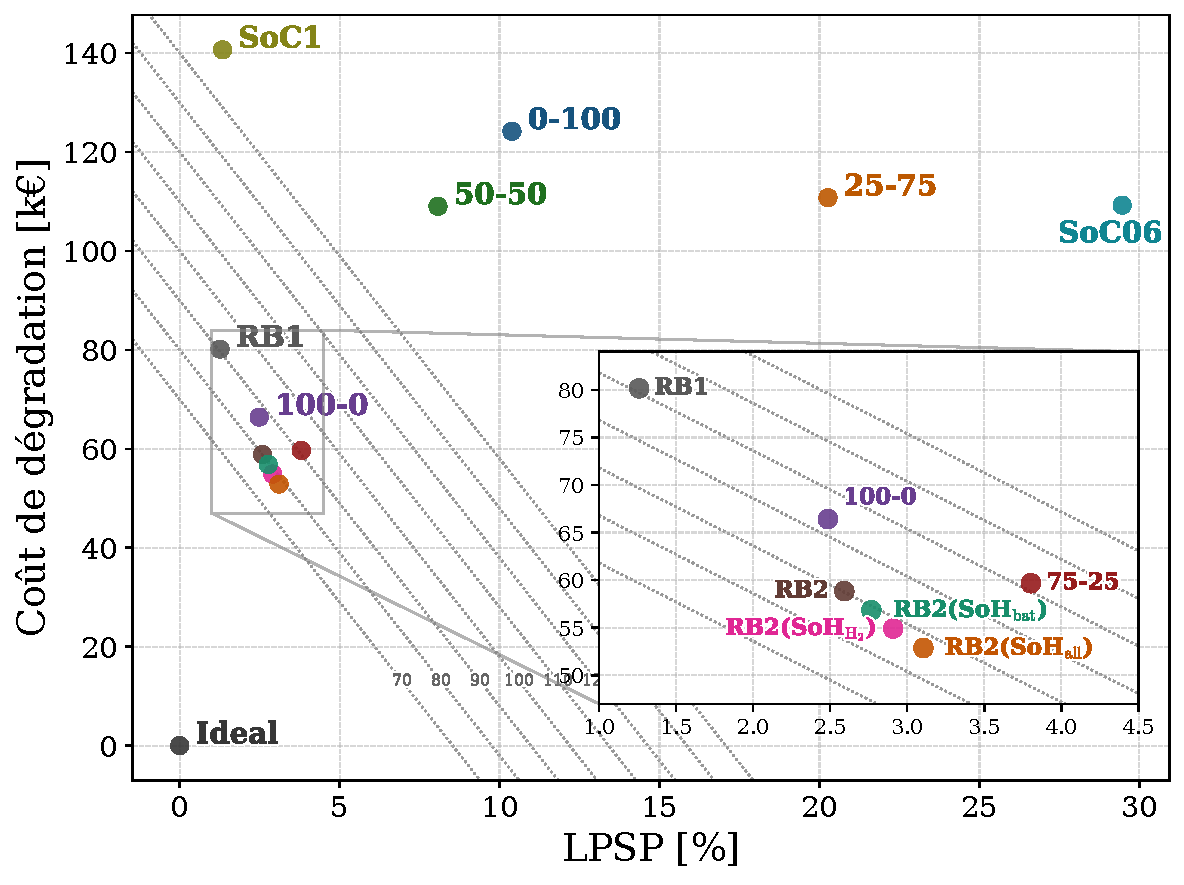
\includegraphics[width=\linewidth]{Chapitre 3/SoH/Figures/pareto_soh_all_isocost.pdf}
    \caption{Positionnement de \RBsohB{} et \RBsohA{} dans le plan de Pareto LPSP--coût de dégradation, avec RB2 et \RBsohH{} (agrandissement sur l'amas RB2 en encart~; lignes d'iso-coût total unifié à VoLL~$=3$~€/kWh, pente $8{,}2$~k€ par point de LPSP).}
    \label{fig:pareto_rb2sohall}
\end{figure}
\FloatBarrier

Dans le plan de Pareto (Figure~\ref{fig:pareto_rb2sohall}), la famille unifiée prolonge le déplacement de \RBsohH{} vers le coin des faibles dégradations~: $52{,}9$~k€ à l'optimum ($g = 0{,}2$), et jusqu'à $50{,}9$~k€ pour $g = 0{,}4$, soit $-10$ à $-13\,\%$ de dégradation par rapport au socle, obtenus par la seule connaissance des états de santé. Le gain $g$ y joue le rôle d'un \emph{curseur de compromis} explicite le long du front~: si l'application impose un plafond de LPSP (par exemple $3\,\%$), la configuration $g = 0{,}1$ constitue le repli naturel. Avec un coût total unifié de $78{,}34$~k€ ($-2{,}2\,\%$ par rapport au socle), \RBsohA{} est la meilleure stratégie \emph{sans prévision} de ce chapitre~; elle servira de base à la stratégie complète construite à la section~\ref{sec:prediction}.
